\section{Python}
\subsection{Première expérimentation}

Dans cette partie, nous allons étudier la consommation énergétique de l'ordinateur lors de la génération d'une image par le biais d'un programme écrit en Python. Nous remplissons donc un tableau avec nos données.
Pour le calcul de l’énergie absorbée, nous utilisons la formule suivante :
\[
E_{\text{absorbée}} = \frac{P_{\text{moy}} \times t_{\text{exécution}} \times 1000}{3600} \text{ (en mWh.)}
\]

Pour le calcul des émissions de \(CO_2\), nous nous basons sur la carte de l'électricité fournie dans le sujet du TP. À la date du TP, les émissions de \(CO_2\) sont de 19~g/kWh d’électricité consommée. Que nous avons arrondi à 20~g/kWh.

\begin{figure}[h]
    \centering
    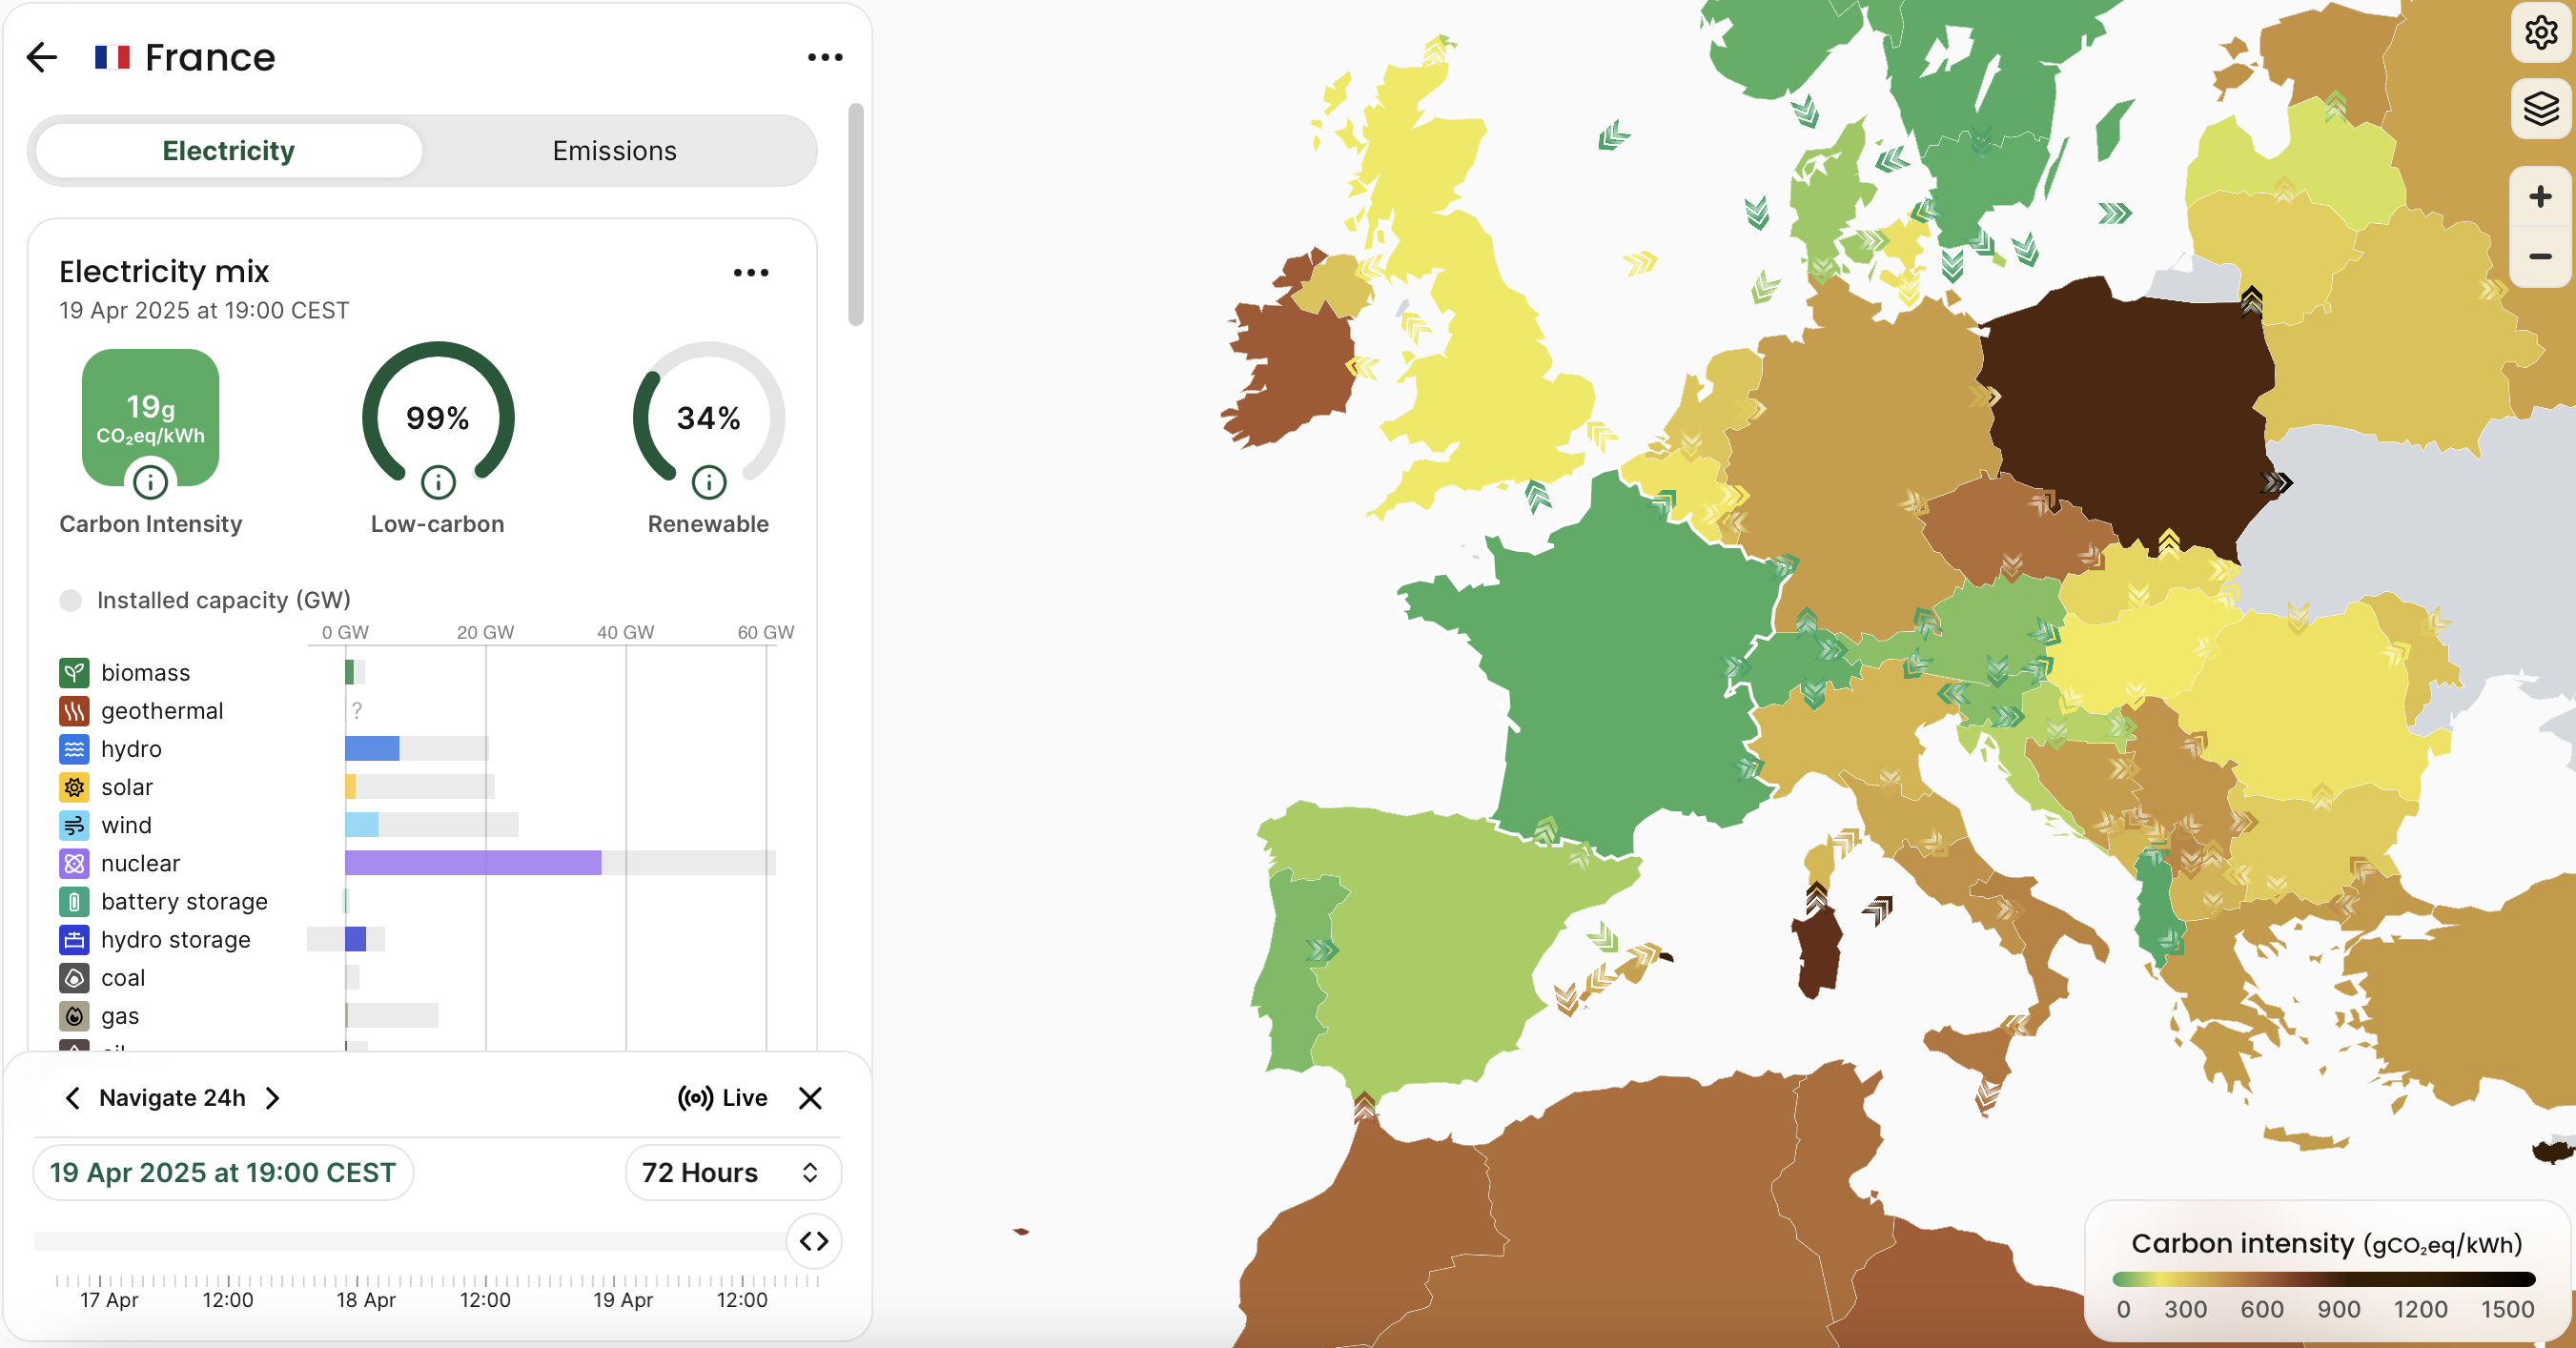
\includegraphics[width=0.8\textwidth]{images/electricity_map.png}
    \caption{Consommation d'électricité en France en temps réel}
\end{figure}


Ainsi, pour calculer les émissions de \(CO_2\), nous multiplions l'énergie absorbée (exprimée en kWh) par l’émission moyenne de \(CO_2\) en France aujourd'hui. On a donc :
\[
CO_{2\text{éq}}(g) = E_{\text{absorbée}} \times 10^{-6} \times 20
\]

Voici les résultats de la première expérimentation..

\begin{figure}[h]
    \centering
    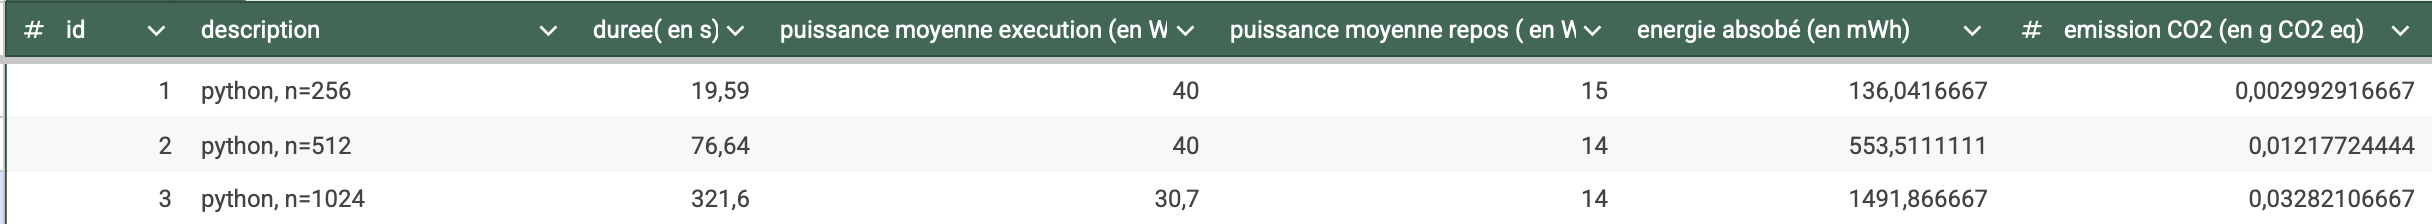
\includegraphics[width=0.85\textwidth]{images/tableur1.png}
    \caption{Résultats pour Python}
\end{figure}

On peut dès le début de la première expérience constater que les temps d’exécution augmentent très rapidement au fur et à mesure que la taille de l’image augmente. On passe par exemple de 11~s de temps d’exécution pour une image \(256 \times 256\) à plus de 5~min pour l’image \(1024 \times 1024\).

\subsection{Seconde expérimentation}

Dans cette seconde expérimentation, nous analysons la consommation énergétique de l’ordinateur pour le même processus, cette fois en utilisant le compilateur \texttt{numba}, qui permet de réduire significativement les temps d’exécution. Le tableau de mesures utilisé reste identique à celui de la première partie.


\begin{figure}[h]
    \centering
    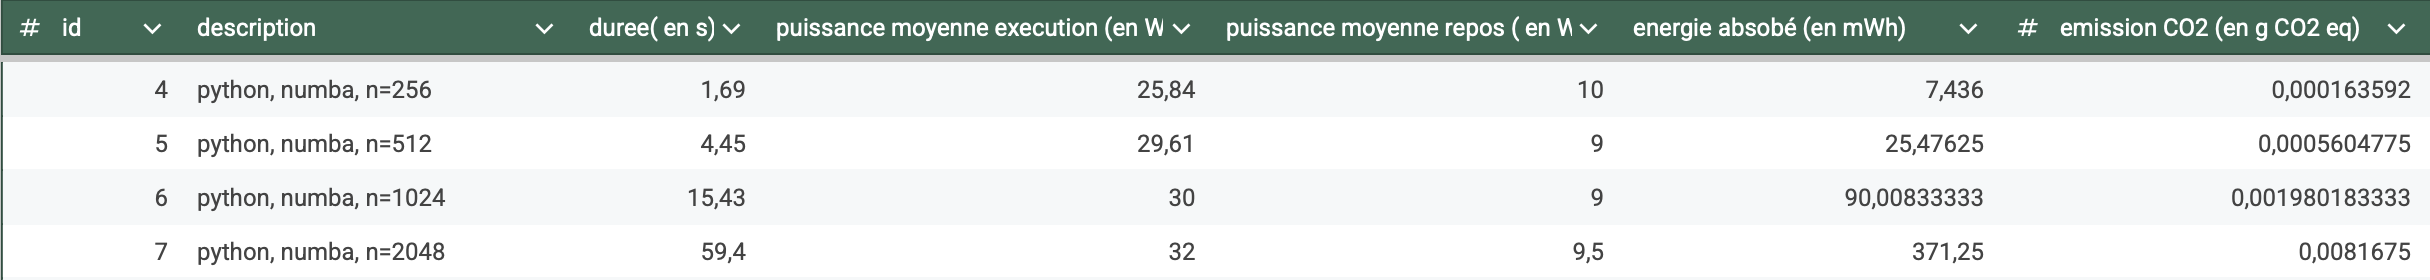
\includegraphics[width=0.85\textwidth]{images/tableur2.png}
    \caption{Résultats pour Python avec \texttt{numba}}
\end{figure}

On peut remarquer que l’ordinateur sur lequel nous faisons l’étude est composé de 24 cœurs logiques.

\begin{figure}[h]
    \centering
    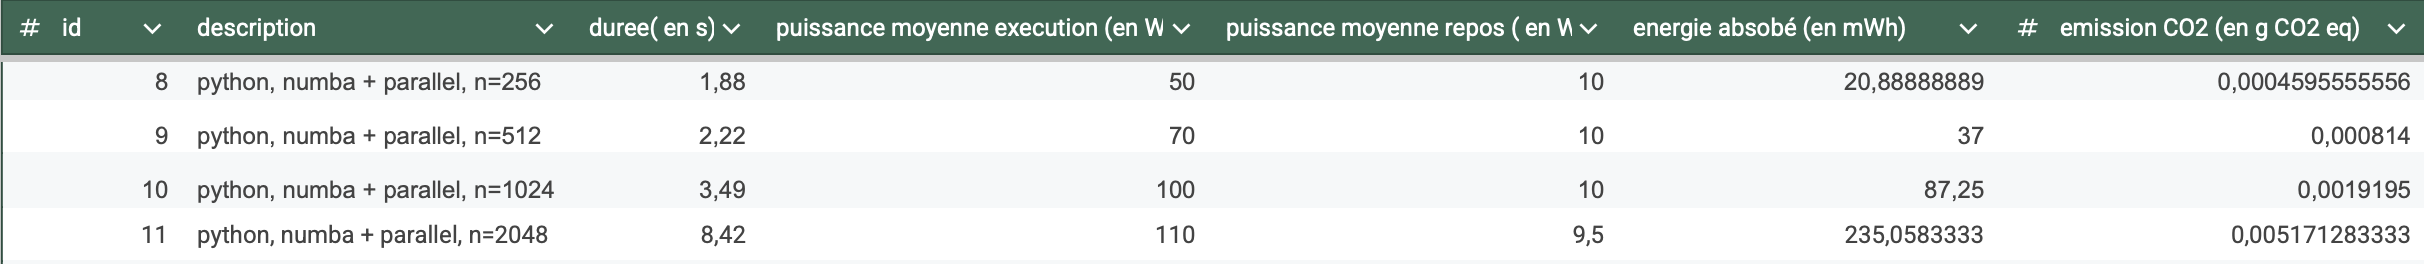
\includegraphics[width=0.85\textwidth]{images/tableur3.png}
    \caption{Résultats pour Python avec \texttt{numba} en parallèle}
\end{figure}

En résumé, l’utilisation du compilateur \texttt{numba} permet de réduire considérablement les temps de calcul sans altérer la précision des résultats. Lorsqu’il est combiné à une exécution en parallèle, les gains en performance sont encore plus marqués. Toutefois, cette accélération s’accompagne d’une consommation énergétique légèrement plus élevée, ce qui met en lumière le compromis classique entre efficacité temporelle et efficacité énergétique.

